% ---- Introduction to Data Section ----

% In this section of the paper, we will describe the data which has been collected and used as the foundation of our later analysis. We will explain our choices when choosing data sources before we delve into the scraping process. Lastly, we will present descriptive statistics of the data used in our analysis. 

% ---- Data Sources ----
\subsection{Data Sources}

\subsubsection{Equity Research Reports}

Through collaborative efforts with Carnegie, DNB Markets, and Pareto Securities, we have compiled a dataset comprising 2,350 ERRs spanning the past five years. The dataset covers the 25 largest companies on the Oslo Stock Exchange (OSE), as determined by market capitalization on the 5th of September 2023.  

% Er gjentagende å si det som nå står i "%" under. Er en gjentagelse av asnittet over
% Our main source of data for this paper has been a compiled set of ERRs disseminated by three Norwegian investment banks. 


When selecting investment banks for our research, we prioritized broad equity research coverage of the firms on the OSE. Carnegie, DNB Markets and Pareto Securities are all among the market leaders in Norwegian equity research, with extensive coverage of the largest companies on the OSE. To access and download the ERRs, we entered into individual agreements with each of the aforementioned investment banks, gaining access to their research portals, namely Carnegie Edge, DNB Alpha, and Pareto Securities Research Portal. The data was manually downloaded and imported into our database.

The dataset extends from January 1st, 2018, to September 4th, 2023. Selecting a five-year time frame was motivated by the practice of investment banks to remove ERRs from their research portals after five years. For instance, DNB Alpha lacks reports before Q4 2018, and although Carnegie and Pareto Securities have some ERRs older than five years, the number of reports significantly diminishes in comparison to recent fiscal quarters\footnote{Detailed further in Figure \ref{fig:reportspub} and Section \ref{sec:descriptive}.}. %Although the ERRs contribute valuable insights, the study faced certain limitations in data collection. Constraints in our agreements with the investment banks limited the number of ERRs we could incorporate, as direct access to their primary databases was not feasible. 

Notably, Fearnley Securities also gave us access to their research portal, but based on the aforementioned criteria for choosing investment banks, we made a strategic decision to exclude their ERRs from our analysis. Fearnley Securities, known for their expertise in the maritime and energy sector, only covers 11 out of the 25 companies we have selected. Including their reports could potentially skew our results, given their sector-specific focus and the uneven coverage of the listed companies. This decision was crucial to maintain the integrity and representativeness of our study, ensuring that our analysis reflects a more balanced and comprehensive view of the market.

%When selecting which covered firms on the OSE we wanted to include, our primary objective was to ensure a representative and robust selection of companies with wide coverage. 
Ensuring a representative and robust selection of companies on the OSE with wide coverage was essential when selecting companies to include in our analysis. Integral to our selection criteria was market capitalization. By focusing on the 25 largest companies on the OSE, we aimed to capture a representative snapshot of the stock exchange's movements. These companies represent 75.96\% of the total OSE market capitalization (\cite{euronext2023}). 

The inherent trade-off between the scope of data and its representativeness was a significant consideration. While a larger number of companies might offer more data points, it is paramount that the data accurately reflects broader market trends. We observed that many smaller companies on the OSE had limited coverage compared to their larger counterparts. This disparity could introduce biases, especially if smaller sample sizes led to an increased number of outliers. By emphasizing larger companies, we not only ensured a more consistent and reliable dataset but also mitigated potential biases. 

We have omitted certain reports from DNB Markets pertaining to DNB and Kongsberg Gruppen due to conflicts of interest. DNB released 29 reports on their own performance creating a situation where their assessment may be influenced by their own stake in the matter, potentially compromising objectivity. Furthermore, DNB acted as an advisor in the potential listing of Kongsberg Digital in 2022, introducing a similar conflict of interest. These conflicts of interest could undermine the impartiality and reliability of two of the reports written in this time period, thus necessitating their omission. In total, the number of reports included in our analysis amounted to 2,319.

The complete set of chosen firms used as a basis for this thesis is presented in Table \ref{tab:selected_companies}. Our selection process was underpinned by the desire for analytical robustness. The utility of choosing this set of firms lies in its ability to offer meaningful insights, and by selecting companies with substantial market capitalization and ample data coverage, we are confident that our set of selected companies provides a comprehensive and accurate reflection of the general use of ERRs in Norway. We posit that the validity of our findings remains consistent despite the significant variance in the number of reports across companies. Some entities have an extensive collection of over 157 reports, while others possess a minimal count of 7. It is important to note that while there are outliers in terms of report volume, the majority of companies exhibit a comparable number of associated reports.

\begin{table}[H]
    \centering
    \small % Reduce font size
    %\setlength{\tabcolsep}{10pt} % Reduce column separation
    %\resizebox{\textwidth}{!}{
    \begin{tabular*}{\textwidth}{@{\extracolsep{\fill}}llccc}
    \toprule
        \textbf{Ticker} & \textbf{Company} & \textbf{Start Date} & \textbf{End Date} & \textbf{Observations} \\ 
      \hline
    ADE & Adevinta & 09.01.2020 & 01.09.2023 &  88 \\ 
      AKER & Aker ASA & 14.05.2018 & 16.06.2023 &  54 \\ 
      AKRBP & Aker BP & 15.01.2018 & 14.07.2023 & 132 \\ 
      AUTO & Autostore & 06.07.2022 & 18.08.2023 &  35 \\ 
      BAKKA & Bakkafrost & 07.05.2018 & 23.08.2023 & 104 \\ 
      DNB & DNB & 01.02.2018 & 12.07.2023 &  94 \\ 
      EQNR & Equinor & 08.02.2018 & 27.07.2023 & 129 \\ 
      GJF & Gjensidige & 26.01.2018 & 14.07.2023 &  101 \\ 
      KOG & Kongsberg Gruppen & 07.02.2018 & 13.07.2023 & 123 \\ 
      LSG & Lerøy Seafood & 27.02.2018 & 24.08.2023 &  96 \\ 
      MOWI & Mowi & 14.02.2018 & 28.08.2023 & 157 \\ 
      NHY & Norsk Hydro & 16.02.2018 & 22.08.2023 & 122 \\ 
      ORK & Orkla & 08.02.2018 & 14.07.2023 & 149 \\ 
      SALM & Salmar & 15.05.2018 & 25.08.2023 & 107 \\ 
      SCHA & Schibsted & 08.02.2018 & 18.07.2023 & 121 \\ 
      SRBNK & SpareBank 1 SR-Bank & 08.02.2018 & 10.08.2023 &  53 \\ 
      STB & Storebrand & 07.02.2018 & 14.07.2023 & 138 \\ 
      SUBC & Subsea 7 & 02.03.2018 & 26.07.2023 &  52 \\ 
      TEL & Telenor & 01.02.2018 & 21.07.2023 & 106 \\ 
      TOM & Tomra & 25.04.2018 & 17.07.2023 &  86 \\ 
      VAR & Vår Energi & 14.07.2022 & 25.07.2023 &  34 \\ 
      YAR & Yara International & 08.02.2018 & 20.07.2023 & 119 \\ 
      FRO & Frontline & 24.04.2019 & 25.08.2023 &  50 \\ 
      HAFNI & Hafnia & 02.02.2023 & 28.08.2023 &   7 \\ 
      WAWI & Wallenius Wilhelmsen & 14.05.2018 & 16.08.2023 &  62 \\ 
        \bottomrule
        \end{tabular*}
    %}
    \caption{Set of Selected Companies}
    \label{tab:selected_companies}
\end{table}

\subsubsection{Financial Data}
For our research, we sourced stock data from Yahoo! Finance. %a reputable online platform that provides comprehensive financial information, including historical stock prices, financial statements, and market data. 
Yahoo! Finance was selected due to its extensive database, ease of access, and reliability of its data (\cite{YahooFinance}). Regarding financial metrics, such as leverage and P/E ratio, we sourced historical data from a Bloomberg Terminal, as this data is not readily available through public APIs \parencite{bloomberg2023}. 

Our primary focus was on the stock prices for this set of companies over a period spanning from 01.01.2016 to 04.09.2023. This amounted to 43,803 data points. The data was extracted using the \textit{tidyquant} package in R. We set our start date for this data collection to be 2 years ahead of our main analysis timeframe, as it allowed us to extract figures which require lagged return data in our analysis.

% ---- Data Cleaning ----
\subsection{Data Cleaning}

\subsubsection{Scraping the PDF Reports}

The ERRs were formatted as PDFs, which is not internally structured for data extraction. The text within the PDFs was scraped to convert it to a usable format, removing extraneous formatting to maintain data integrity. To accommodate Scandinavian letters in company names, the PDF encoding was adjusted to UTF-8. While this does not affect sentiment analysis, as the ERRs are written in English, it enhances the readability of the data, where company names serve as a sorting token. The encoded textual data was added to our main corpus for further processing.

As the PDFs lack metadata, scraping the raw textual data in our corpus for key information, such as target price and recommendation, is important. One of the complexities of the data cleaning process was the lack of uniformity in the report structures. Each company have their unique formatting style for their reports, making it infeasible to employ a universal cleaning script. Consequently, the scraper was tailored to accommodate the specific style of each investment bank, ensuring the precision of data extraction.

An essential piece of information for our analysis was the report date, which is not available in a given reports metadata. We observed that most reports contained a statement similar to: “This report was completed and disseminated 14 Oct 2022: 17:40 CET”. To capture the date, a function was written that scanned the first 20 lines of the PDF, extracting any recognizable date. The extracted dates were standardized, and their occurrences counted. In instances of multiple identified dates, the date with the highest frequency was selected. In the event of a tie, the observed date closest to the current date was selected to ensure relevant and accurate data. For other data points, such as recommendation and target price, a similar approach was employed. 

The reports contained mandatory sections which investment banks are legally bound to include. These sections elucidate the legal constraints of their recommendations. Given their consistent nature across reports, these sections were excluded. This decision was made to prevent bias in our analysis, focusing on the unique and pertinent content of each report. Upon completion of the data extraction and cleaning process, the refined data and the sanitized PDF text were stored in a data frame. %setting the stage for subsequent analyses.

\subsubsection{Cleaning the Financial Data}
The data gathered from Yahoo! Finace was directly loaded into a data frame for further processing. The Bloomberg Excel add-on was used to automate the process of downloading the necessary fiscal data for each firm, and converted it into a structured data format. It is worth noting that data from reputable sources like Yahoo! Finance and Bloomberg often comes well-structured and largely free from glaring discrepancies. However, it is a cardinal rule in data analysis to never trust data at face value. Hence, even though the data was formatted to our expectations upon download, we reviewed the data thoroughly. We found no large discrepancies in the downloaded data. We adjusted our stock prices for stock splits and dividends, as these events can introduce discontinuities in time series data. By adjusting for such events, we ensured that our dataset maintained its continuity and comparability throughout the chosen analysis period. 
\begin{table}[H]
    \centering
    \small
    %\setlength{\tabcolsep}{21pt} % Reduce column separation
    \resizebox{\textwidth}{!}{
    \begin{tabular*}{\textwidth}{@{\extracolsep{\fill}}lccc@{}}
    \toprule
        \textbf{Ticker} & \textbf{Company} & \textbf{Stock Split Date} & \textbf{Split Ratio} (\(\kappa_t\)) \\ 
    \midrule
          TOM & Tomra & 27.05.2022 & 2:1 \\ 
          VAR & Vår Energi & 15.02.2023 & 11:10 \\ 
    \bottomrule
    \end{tabular*}
    }
    \caption{Stock Split Information}
    \label{tab:stock_split}
\end{table}
Yahoo! Finance incorporates stock split adjustments in its historical price data. Conversely, previously published ERRs do not undergo similar updates. Consequently, it becomes imperative to rectify the provided target prices in accordance with the stock split ratio. As a result of this adjustment, the target prices for Tomra and Vår Energi, prior to the stock split date, are now suitably transformed in order to keep the ratio the target prie and share price equal equal to when the report was published. The stock split ratios can be found in Table \ref{tab:stock_split} and the adjusted target price \(\hat{P}_{a,t}^{'}\) is calculated as given by Equation \ref{eq:split}
\begin{equation} \label{eq:split}
    \hat{P}_{a,t}^{'}=\frac{\hat{P}_{a,t}}{\kappa_t}
\end{equation}

where \(\hat{P}_{a,t}\) denotes the target price of investment banks \(a\) in time \(t\) and \(\kappa_t\) the split ratio of a stock\footnote{We treat the split ratio \(\kappa_t\) of n:m as $\frac{n}{m}$.}. 

% ---- Final Dataset ----

% In this section we are going to present the various explanatory variables,
% response variables and the explanatory variables (trend variables)

\subsection{Final Dataset}

\subsubsection{Sentiment Score}

To assess the textual sentiment, we employed a lexicon-based approach\footnote{We go into detail about this implementation in Section \ref{sec:dict}.}. This method relies on a predefined dictionary or lexicon, where each word is associated with a polarity score. The sentiment is determined by aggregating the scores of its constituent words, as shown in Equation \ref{eq:sentiment_score} 
\begin{equation}
\label{eq:sentiment_score}
    s_q = \frac{\gamma^{pos}_{q_i} - \gamma^{neg}_{q_i}}{\gamma^{pos}_{q_i} + \gamma^{neg}_{q_i}}
\end{equation}
where the textual sentiment score \(s\) of report \(q_i\) is set as \(s_q\). This score is defined as the fraction of the difference between total positive tokens \(\gamma^{pos}_{q_i}\) and total negative tokens \(\gamma^{neg}_{q_i}\), and the sum of total positive and negative tokens. This produces a normalized sentiment score defined as a real number within the closed interval \([-1,\:1]\).

A notable advantage of this approach is its independence from labeled training data. We base our sentiment score on the work done by Feuerriegel et al. \parencite*{feuerriegel2015information} with some slight modifications. As the ERRs contain tables and graphs, we opted out of standardizing the score based on word count. Although we lose some ability to measure the strength of the sentiment in a report, we believe that the negative effects of including a high degree of noise in our score would outweigh the benefits. We found that the number of loaded\footnote{We define loaded words as the sum of positive and negative words in a report, i.e \(\gamma^{pos}_{q_i} + \gamma^{neg}_{q_i}\).} words were highly correlated with the number of total words in a report, which tells us that we keep some ability to measure sentiment strength.


\subsubsection{Target Ratio}

% To facilitate a meaningful comparison of target prices, regardless of the price level, we employ a relative measure by dividing each target price by the stock price one day prior to the ERR being published, namely the \textit{target ratio}. We utilize the stock price from the day prior to the target valuation to ensure that fluctuations in the target price do not impact the intraday stock price.

To compare target prices, we employ the relative measure \textit{target ratio} \(\rho_t\), shown in Equation \ref{eq:TargetRatio}, drawing inspiration from De Vincentiis \parencite*{de2010accuracy}. By dividing each target price \(\hat{P}_{a,t}^{'}\) in time \(t\) by the stock price one day prior to the ERR being published $P_{t-1}$, we allow for a consistent assessment of target prices regardless of varying stock levels, and ensure that new information contained in the ERR does not impact the intraday stock price. 
\begin{equation}
\label{eq:TargetRatio}
    \rho_t=\frac{\hat{P}_{a,t}^{'}}{P_{t-1}}
\end{equation}

%The target ratio is denoted as \(\rho_t\) where \(t\) is time. The target price in time \(t\) is denoted as \(\hat{P}_{a,t}^{'}\), whilst stock price one day prior is denoted as \(P_{t-1}\).

% Explain how we will use this (we have it as the dependant variable in a sort of benchmark regression later)

\subsubsection{Explanatory Variables}

We incorporate the \textit{RETURN\_3M}, \textit{MACD}, and \textit{RSI} as explanatory variables, adeptly capturing short-term market trends. We decided to only use a 3-month simple return as time frames such as 1-week and 12-month returns cause multicollinearity issues, correlating with the RSI and the 3-month return respectively.

\subsubsection{Control Variables} \label{sec:controlvariables}

%thus affecting the textual sentiment

Controlling for firm-specific differences impacting opinions toward a stock, thus affecting the sentiment score, we have added several control variables. Note that some of the variables are log-transformed to address issues of skewness and heteroscedasticity, ensuring a more accurate representation of their influence on the dependent variable \parencite{virginiaInterpretingTransformations}.

Firm size has in relevant literature been used as a proxy for the extent of publicly available information about a company \parencite{das1998earnings}. Larger firms tend to have a more extensive and accessible pool of data, which can impact the accuracy of forecasts. Moreover, larger companies often garner more attention from investors, leading to a greater depth of coverage \parencite{fortin2007analyst}. In line with Al-Awadhi et al. \parencite*{al2020death}, we control for firm size through the market capitalization of a firm, \textit{log\_market\_cap}. 

Existing literature finds a significant correlation between firm age and beta, indicating that younger companies tend to exhibit higher levels of risk and volatility \parencite{chincarini2020beta}. This, in turn, can influence target price estimations, as beta is a critical factor in determining a stock's expected return. Furthermore, younger companies, often in need of external financing to sustain growth, may be incentivized to exceed earnings expectations to attract investor attention and secure necessary capital \parencite{coad2016innovation,loderer2010firm}. We account for the temporal aspect of a company's post-IPO tenure through the natural logarithm of years since IPO-date, \textit{log\_time\_on\_OSE}. %Note that Euronext does not publicly display records of stock data before the 19th of January 2000, which in turn skews the IPO date of companies listed before this date.

Addressing potential bias stemming from unobserved time-invariant factors is important. Variations in reporting standards or other idiosyncrasies can influence the dependent variable. By introducing \textit{analyst} as a dummy variable for investment bank \(a\), %fixed effect estimator
we effectively account for unobserved heterogeneity. %, allowing us to isolate and quantify the impact of other independent variables accurately. 
The dummy variables \textit{analystDNB} and \textit{analystPARETO} are incorporated, making Carnegie the reference group. 

Next, we incorporate a dummy variable \textit{dividend} for dividend payments within the last 30 days. Capstaff et al. \parencite*{capstaff2004share} document significant abnormal returns on the OSE following a dividend announcement, providing support for dividend signaling theory in Norway. %Thus, we control for this, reducing potential omitted variable bias (OVB).

The price-to-earnings (P/E) ratio is a valuation multiple of the share price divided by the earnings per share, providing a measure of how much a company is valued relative to their earnings. While reading the ERRs in our dataset, it becomes evident that P/E is an essential part of their target price, explicitly using P/E and forecasted P/E to value companies. Thus, we incorporate the control variable \textit{log(pe\_ratio)}.

Dechow \& You \parencite*{dechow2020understanding} find that increased financial leverage causes equity research analysts to assume higher returns implied through their target price. As this might impact their assessment of the stock, hence the textual sentiment, we control for \textit{financial\_leverage}.

Volatility influences the range of target prices, reflecting the inherent uncertainty in stock performance \parencite{cho2014effect}. Employing a 1-year volatility estimate coincides with the forecast horizon in ERRs, thus accounting for short to medium-term market dynamics. While sophisticated models like GARCH(1,1) can account for excess kurtosis in stock returns, the impact on our volatility estimates would likely be marginal. Thus, we opt for a simplistic approach. The control variable \textit{volatility} is calculated through three steps. The first step calculates the continuously compounded daily return $u_i$, as this is preferred for stock volatility \parencite{investopediaUsingHistorical}. %Research finds that the distribution of logarithmic monthly standard deviations, derived from daily returns, closely resembles a Gaussian distribution \parencite{andersen2001distribution}, aligning with the findings of Taylor \parencite*{taylor2008modelling} and French et al. \parencite*{french1987expected}. Thus, 
The second step estimates the daily standard deviation $\sigma_n$ on a rolling 30-day basis, while the third and final step annualizes it accordingly with Höhler \& Lansink \parencite*{hohler2021measuring}. The three steps are presented in Equation \ref{eq:vol1}, \ref{eq:vol2}, and \ref{eq:vol3}.
%sample variance m-1
% Fix this notation
\begin{equation}
\label{eq:vol1}
    u_i = ln\left(\frac{P_i}{P_{i-1}}\right)
\end{equation}
\begin{equation}
\label{eq:vol2}
    \sigma_n=\sqrt{\frac{1}{m-1}\sum_{i=1}^{m}(u_{n-i}-\overline{u})^2}
\end{equation}
\begin{equation}
\label{eq:vol3}
    \sigma_{a}=\sigma_{n}*\sqrt{252}
\end{equation}

%Additionally, considering implied volatility, which leverages option prices to project future volatility, aligns with analysts' objectives. However, we opt for the simplistic approach, %to mirror the fundamental thought process of most humans as this straightforward measure remains widely embraced due to its intuitive nature and accessibility \textcolor{red}{(kilde)}. 

Considering the recent 5-year period characterized by heightened market uncertainty surrounding the COVID-19 pandemic, impending rate hikes, war, and recessionary fears, the VIX-index serves as a great variable to account for the extraordinary volatility. Further, literature finds that investment banks tend to issue more optimistic earnings forecasts and buy recommendations under market uncertainty, as measured by the VIX \parencite{chang2017analyst}. Thus, incorporating the control variable \textit{VIX} ensures that the model adequately captures the nuanced effects, providing a more robust and reliable analysis.

Analyst opinions tend to exhibit a degree of \textit{stickiness} over time, driven by a reluctance to abandon beliefs \parencite{bouchaud2019sticky}. Studies find that investment banks exhibit an excessive adherence to long-term trends, leading to a lag in their response to short-term shifts \parencite{filiz2021sticky}. Thus, we control for the sentiment from the last ERR, \textit{sentiment\_1lag}, and the \textit{target\_ratio\_1lag}, accounting for stickiness.%we ensure a more balanced assessment of the current sentiment.

% TENK PÅ FORSKJELLEN PÅ DIVIDEND ANNOUNCEMENT OG DIVIDEND PAID --> Bør kanskje gjøre noe med dette


% This paper is much better \cite{capstaff2004share} as it looks at the oslo stock exchange and find abnormal returns within the confides of strong form of Efficient Markets Hypothesis

%\subsubsection{Interaction Terms}

%It is important to consider potential joint effects amongst our variables on sentiment, such as dividends and firm size. Tekin \parencite*{tekin2020firm} suggest that smaller firms issuing dividends may yield stronger signaling effects compared to larger companies \textcolor{red}{partially due to higher information asymmetry}. However, our data is based on the 25 biggest companies on the OSE, potentially limiting the relevance of this interaction effect within our dataset. We have opted for a simplified model, as we do not perceive any critical interdependencies at play. Hence, we have chosen not to incorporate any interaction terms.

\subsubsection{Presenting Model Dataset}

% Insert main text here
% ----

Following the identification and definition of the dependent, explanatory, and control variables, we present the full dataset which forms the basis of our analytical framework. Table \ref{tab:fulldataset} illustrates the complete array of data employed in our empirical analysis\footnote{A set of summary statistics for all variables can be found in Appendix \ref{appendix:finaldata}.}.

% ----

\begin{table}[H]
    \centering
    \begin{tabularx}{\textwidth}{ll}
    \toprule
       \textbf{Variable Name}  & \textbf{Definition} \\ \hline \\
       \textbf{Dependent Variables} & \\ \hline
       sentiment & Our calculated sentiment score \\
       target\_ratio & Target price divided by share price at \(t-1\) \\ \\
       \textbf{Explanatory Variables} & \\ \hline
       RSI & Relative Strength Index \\
       MACD & Moving Average Convergence Divergence \\
       RETURN\_3M & 3 month simple return of stock  \\ \\
       \textbf{Control Variables} & \\ \hline log(market\_cap) & Market cap of company \\
       log(time\_on\_OSE) & Years since IPO \\
       analyst & Dummy variable for investment bank \\
       dividend & Dummy variable for dividend paid last 30 days \\ 
       log(pe\_ratio) & Price to earnings ratio \\
       financial\_leverage & Debt divided by equity \\
       volatility & 1-year annualized rolling volatility estimate \\ 
       VIX & Volatility index \\ 
       sentiment\_1lag & Sentiment in previous ERR \\ 
       target\_ratio\_1lag & Target price divided by share price for ERR in \(t-1\)
       \\ \bottomrule
    \end{tabularx}
    \caption{Variables in the Model Dataset}
    \label{tab:fulldataset}
\end{table}

% ---- Descriptive Statistics ----
\subsection{Descriptive Statistics} \label{sec:descriptive}

Figure \ref{fig:reportspub} shows the distribution of ERRs by fiscal quarter. As the number of reports from 2018 Q3 and before are not as well represented in our dataset, we see that the investment banks tend to remove reports which are more than five years old from their database which is available to customers. DNB seem to be more strict in their removal policy, as we find no ERR reports which is older than five years.

\begin{figure}[H]
        \centering
        \includesvg[width=\textwidth]{Images/reportsQ.svg}
        \caption{Number of Equity Research Reports Published per Quarter}
        \label{fig:reportspub}
    \end{figure}
    
For the sentiment score, defined in Section \ref{eq:sentiment_score}, we expect to find a distribution which is comparable to a Gaussian distribution based on the assumptions of the central limit theorem. In Figure \ref{fig:sentdist} we find that the sentiment score is normally distributed with a mean of around -0.14, although this distribution changes if we differentiate between the investment banks. We find that each investment bank follows quite different distributions, with DNB and Pareto having comparable means, while Carnegie exhibits a much more positive distribution in terms of sentiment. This could be explained by varying policies or attitudes within each investment bank, which could be confirmed by analyzing other similar metrics. If these results are not reproducible, it could point to a weakness in our sentiment score. Additionally, the negative mean sentiment score could indicate that even though the majority of recommendations are \textit{BUY}, the sentiment of the reports tend towards the negative end of the scale. This negative bias could be explained by the choice of sentiment dictionary, as the LM dictionary contains 6.75 times more negative words than positive words, which could skew the average sentiment of the reports.

\begin{figure}[H]
    \centering
    \adjustbox{max width=\textwidth}{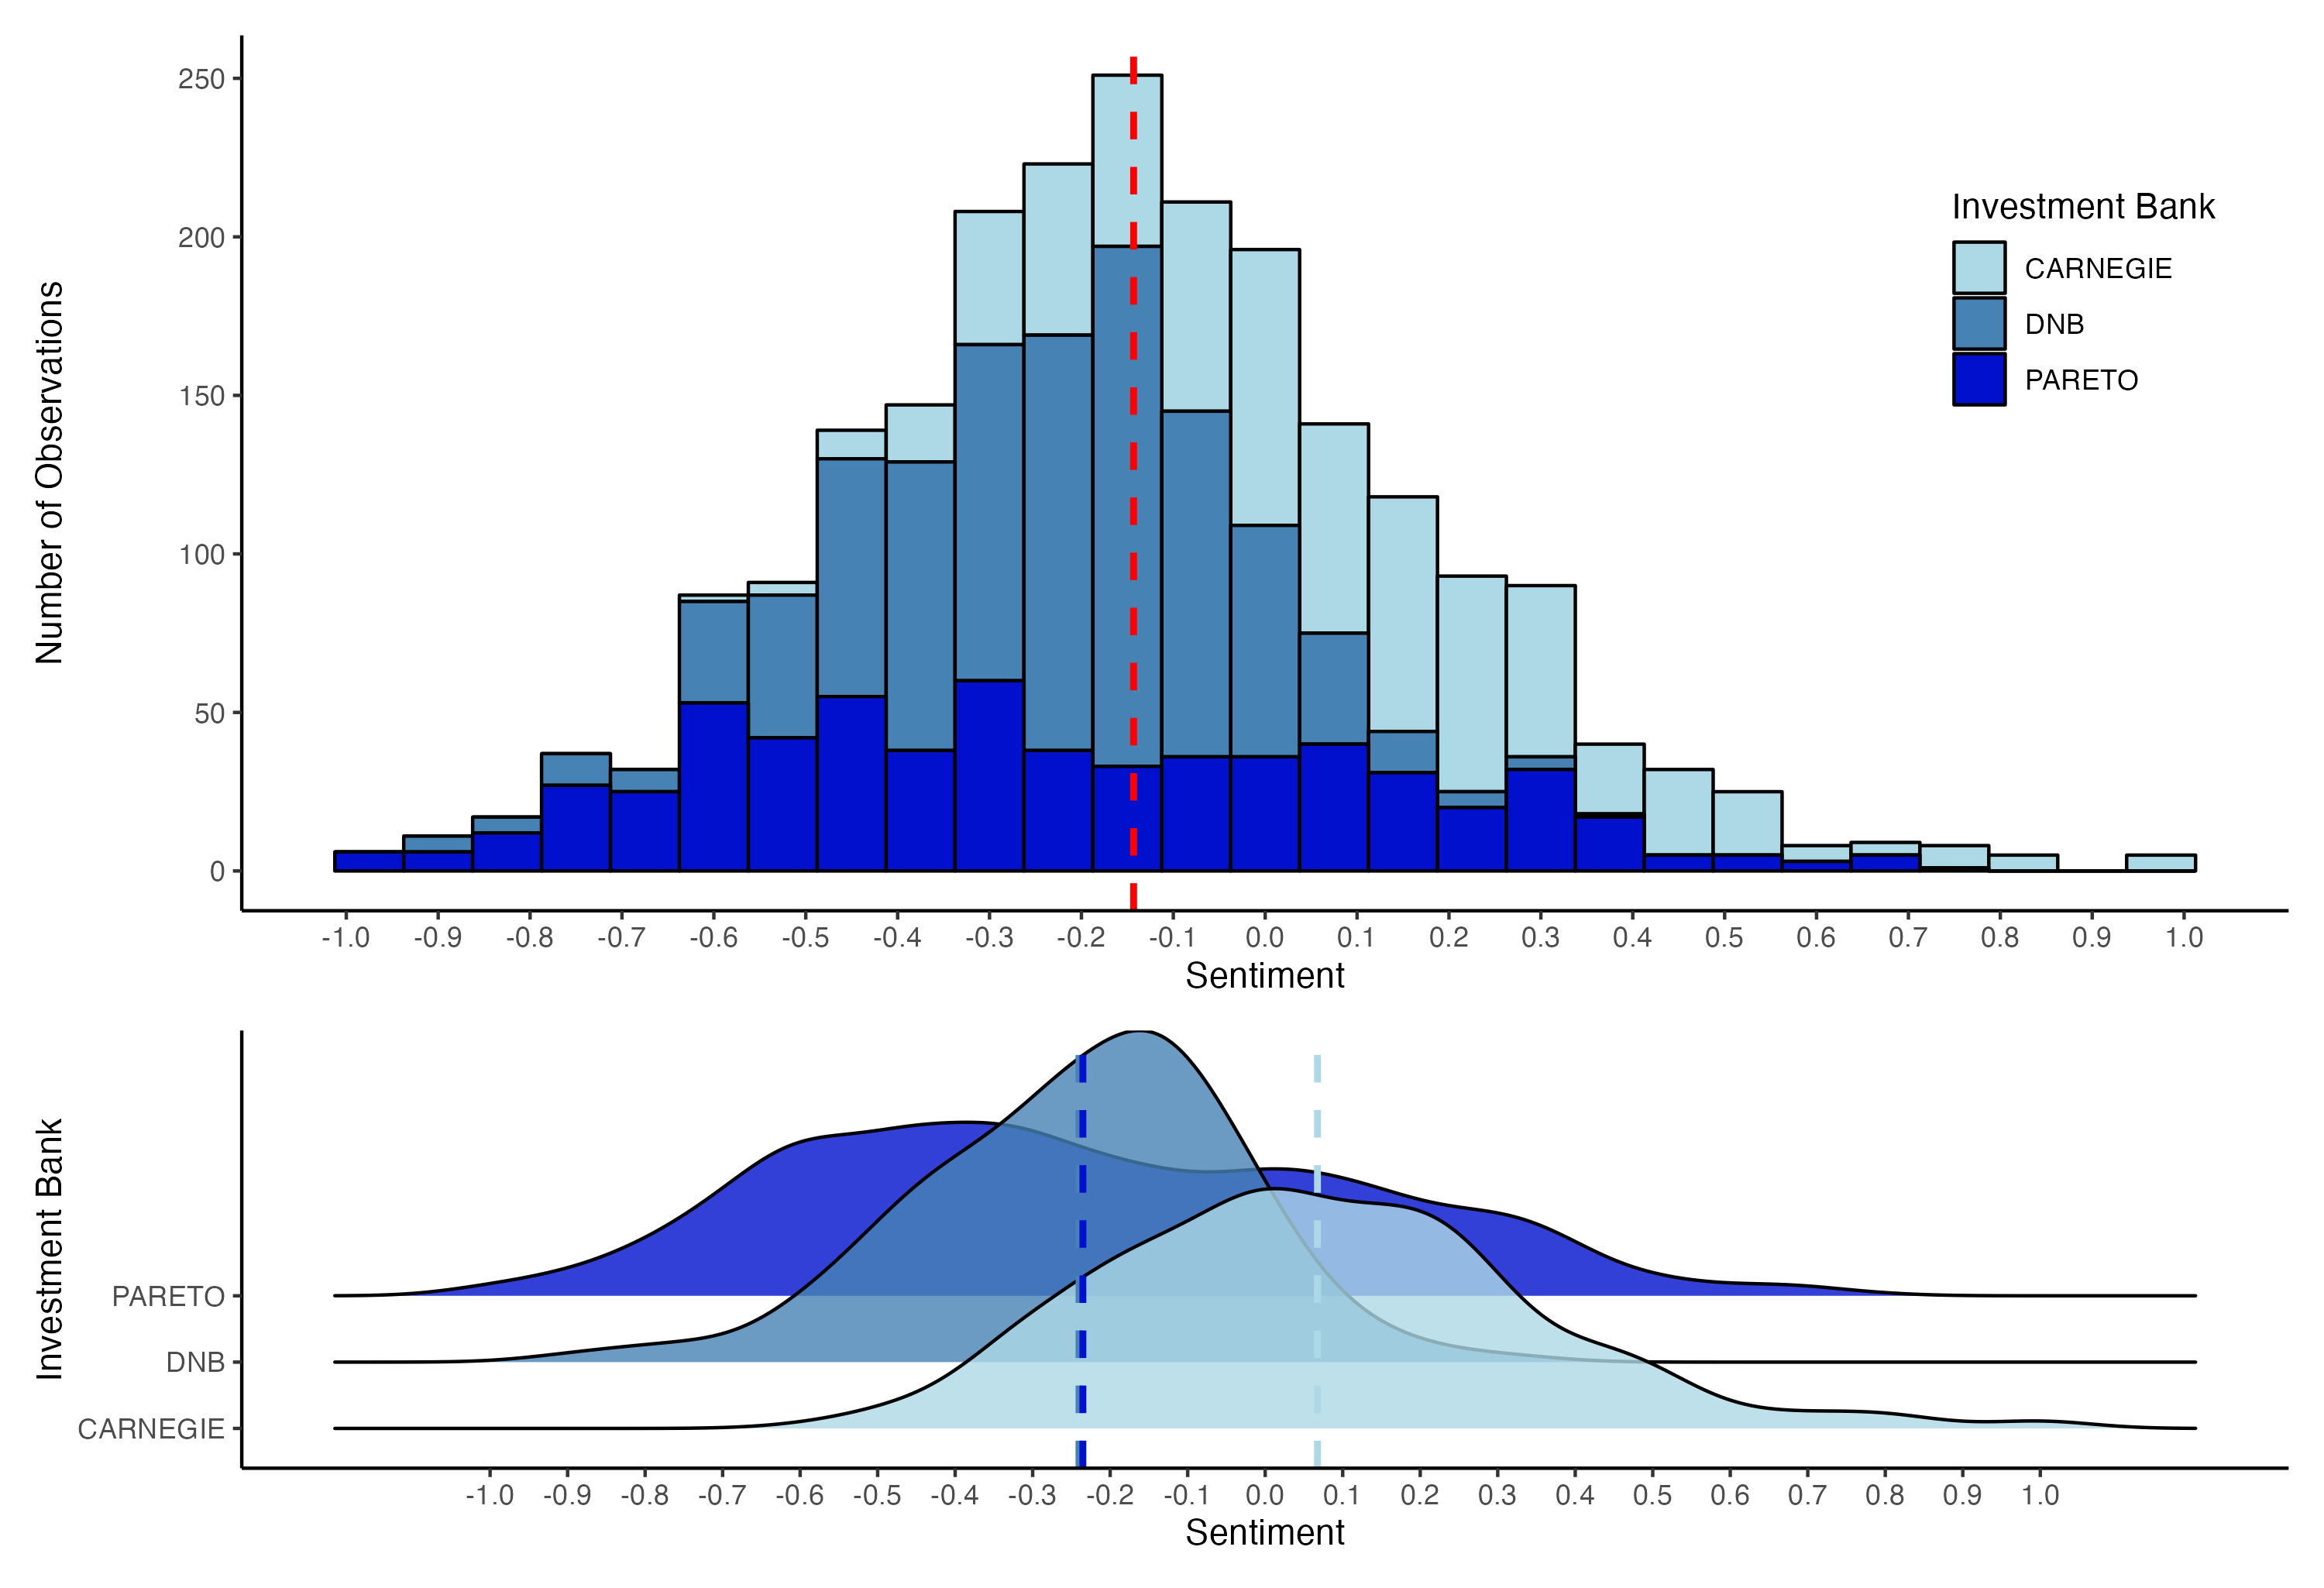
\includegraphics{Images/sentiment_dist.png}}
    \caption{Textual Sentiment Score Distributions by Investment Bank}
    \label{fig:sentdist}
\end{figure}


% Target ratio over time
In Figure \ref{fig:reccomendationstime}, we analyze the change over time of recommendation distributions from three investment banks. Statistical analysis reveals distinct recommendation patterns: Carnegie exhibits a significantly elevated \textit{BUY}-ratio, driven by a relatively low \textit{HOLD}-ratio, and a moderate \textit{SELL} inclination. DNB, characterized by a higher prevalence of \textit{HOLD} and \textit{SELL} recommendations, shows a pronounced sentiment distribution, seen in Figure \ref{fig:sentdist}. Pareto demonstrates a dominant \textit{HOLD}-ratio with fewer \textit{BUY} and \textit{SELL} suggestions, correlating with a flatter sentiment distribution in Figure \ref{fig:sentdist}, indicating a more responsive reporting approach compared to the other two companies. These distributions show us that there is a high probability of there being structural differences in how the reports are written between each investment bank, which could be the root cause behind the difference in distribution and mean of the sentiment scores.

\begin{figure}[H]
        \centering
        \includesvg[width=\textwidth]{Images/rec_dist.svg}
        \caption{Target Ratio and Recommendation Distributions Between Investment Banks}
        \label{fig:reccomendationstime}
    \end{figure}

%\subsection{Data Quality and Other Considerations}

